\documentclass[../../InformazioneQuantistica.tex]{subfiles}

\begin{document}
\section{Canali quantistici}
\lesson{8 \reddot}{21/3/2019}
Per \textbf{canale quantistico} si intende un qualsiasi processo fisico, non generalmente unitario, che trasforma lo stato $\rho_S$ di un certo sistema $S$ in uno stato $\rho_S'$. In particolare stati puri possono essere mappati in stati misti.\\

Nella pratica, i canali quantistici consentono di modellizzare \textbf{sistemi aperti}, in cui si ha interazione tra il sistema $S$ che si controlla e l'ambiente $E$ circostante. Sperimentalmente, infatti, nessun sistema può essere completamente isolato da ciò che lo circonda, e le correlazioni che vengono a crearsi tra $S$ ed $E$ tendono ad introdurre \textit{rumore} in $S$, che finisce per rendere tale stato \textit{inutilizzabile}.\\
Nello specifico l'interazione con l'ambiente è all'origine del fenomeno di \textbf{decoerenza}, che \textit{distrugge} lo stato di sovrapposizione quantistica di $S$, riducendolo ad una \textit{mistura statistica}.\\
In un certo senso, la decoerenza funge da ponte tra il mondo quantistico, in cui vale il principio di sovrapposizione, e il mondo classico, in cui stati mutualmente esclusivi non possono esistere contemporaneamente.

\subsection{Decoerenza di un qubit}
Il caso più semplice si ha quando partiamo da uno stato puro $\rho_S = \ket{\psi}\bra{\psi}$, con $\ket{\psi}$ stato generico di un singolo qubit:
\begin{align*}
\ket{\psi}=\alpha\ket{0} + \beta \ket{1} \Rightarrow  \rho_S = \ket{\psi}\bra{\psi} = \begin{pmatrix} |\alpha|^2 & \alpha \beta^* \\ \alpha^* \beta & |\beta|^2 \end{pmatrix}
\end{align*}
Il processo di \textbf{decoerenza} annulla i termini di coerenza, cioè quelli fuori dalla diagonale principale di $\rho_S$:
\begin{align*}
\rho_S \mapsto \rho_S' =  \begin{pmatrix}|\alpha|^2 & 0 \\ 0 & |\beta|^2
\end{pmatrix}
\end{align*}
Tale trasformazione può essere schematizzata dall'azione di una CNOT, che usa come qubit di controllo il $\rho_S$, e lo correla con lo stato $\ket{0}_E$ dell'ambiente:
\begin{figure}[H]
\centering
\tikzset{every picture/.style={line width=0.75pt}} %set default line width to 0.75pt        
\begin{center}
\begin{tikzpicture}[x=0.75pt,y=0.75pt,yscale=-1,xscale=1]
%uncomment if require: \path (0,300); %set diagram left start at 0, and has height of 300

%Straight Lines [id:da5839193375924283] 
\draw    (230,120) -- (390,120) ;


%Straight Lines [id:da5250417297428058] 
\draw    (230,170) -- (390,170) ;


%Straight Lines [id:da6806435798614072] 
\draw    (310,120) -- (310,170) ;


%Flowchart: Or [id:dp38998241497199526] 
\draw   (300,170) .. controls (300,164.48) and (304.48,160) .. (310,160) .. controls (315.52,160) and (320,164.48) .. (320,170) .. controls (320,175.52) and (315.52,180) .. (310,180) .. controls (304.48,180) and (300,175.52) .. (300,170) -- cycle ; \draw   (300,170) -- (320,170) ; \draw   (310,160) -- (310,180) ;

% Text Node
\draw (217,120) node   {$\rho_S$};
% Text Node
\draw (217,170) node   {$|0\rangle_E$};
% Text Node
\draw (403,120) node   {$\rho'_S$};


\end{tikzpicture}
\end{center}
\caption{Schema dell'azione CNOT che \q{distrugge} le coerenze di $\rho_S$\label{fig:qubit-CNOT}}
\end{figure}
Vediamo come. Lo stato iniziale del sistema qubit-ambiente è dato da:
\begin{align*}
\ket{\psi_0}_{SE} = \ket{\psi}_S\otimes \ket{0}_E = (\alpha\ket{00}+\beta\ket{10})_{SE}
\end{align*}
L'azione della CNOT lo porta a $\ket{\psi_1}$:
\begin{align*}
\ket{\psi_1}=\alpha\ket{00}_{SE}+\beta\ket{11}_{SE}
\end{align*}
In altre parole, quando il sistema è nello stato $0$, lo stato dell'ambiente rimane imperturbato, ma quando il qubit $S$ è nello stato $1$, il qubit di $E$ viene invertito.\\
La $\ket{\psi_1}$ è uno stato non separabile, cioè entangled: la CNOT ha quindi \textit{correlato} $S$ ed $E$.\\

Si verifica ora che $\rho_S'$ ottenuta eseguendo la traccia parziale di $\rho_1 = \ket{\psi_1}\bra{\psi_1}$ ha i termini di coerenza nulli:
\begin{align*}
\rho'_S = \underset{E}{\op{Tr}} \ket{\psi_1}\bra{\psi_1} = \begin{pmatrix}|\alpha|^2 & 0\\ 0 & |\beta|^2\end{pmatrix}
\end{align*}
Fisicamente ciò significa che, poiché lo stato di $S$ dipende da quello di $E$, una misura su $S$ in cui ? %[TO DO] Continuare da qua e finire

\marginpar{\danger Parte non ancora ricontrollata}
L'azione della CNOT schematizza idealmente l'interazione tra il qubit $S$ e l'ambiente $E$: si può quindi affermare che facendo interagire i due sottosistemi si \textit{distrugga} la coerenza di ciascuno. Perciò, se vogliamo effettuare operazioni quantistiche con qubit entangled, è necessario realizzare un sistema completamente isolato dall'esterno - cosa molto complessa nella pratica.\\

Possiamo vedere l'evoluzione \q{che distrugge le coerenze} dal solo punto di vista del primo sottosistema, tramite opportuni operatori di Kraus $\{E_k\}$:
\begin{align}
\rho_S \mapsto \rho'_S = S(\rho) = \sum_{k} E_k \rho E_k^\dag \qquad \sum_k E_k^\dag E_k = \bb{I}
\label{eqn:ev-kraus}
\end{align}
Avevamo visto che una $\rho_S$ generica di un qubit può essere scritta nella base $\{\bb{I}, \hat{\sigma}_i\}$ delle matrici hermitiane $2\times 2$:
\begin{align}
\rho = \frac{1}{2}(\bb{I}+\vec{r}\cdot \vec{\sigma}) \Rightarrow  \rho'=\frac{1}{2}(\bb{I}+\vec{r}\,'\cdot \vec{\sigma})
\label{eqn:ev-vector}
\end{align}
dove $\vec{r}$ e $\vec{r}\,'$ sono due vettori nella sfera di Bloch (non necessariamente sulla sua superficie, come avviene nel caso degli stati misti).\\
Osservando l'evoluzione da tale punto di vista, otteniamo una \textbf{trasformazione affine}:
\begin{align*}
\vec{r} \mapsto \vec{r}\,' = M\vec{r} + \vec{c}
\end{align*}
per una certa matrice $M_{3\times 3}$ e vettore $\vec{c} \in \bb{R}^3$.\\
Anche gli operatori di Kraus possono essere scritti nella stessa base:
\begin{align*}
E_k = \gamma_k \bb{I} + \sum_{l=1}^3 a_{kl}\hat{\sigma}_l
\end{align*}
Uguagliando allora la (\ref{eqn:ev-vector}) con la (\ref{eqn:ev-kraus}), dopo vari passaggi di algebra si giunge ad espressioni esplicite per $M$ e $c$:\marginpar{\danger Gli indici potrebbero essere molto errati}
\begin{align*}
M_{jk} &= \sum_{l=1}^3 \left\{ a_{lj}a_{lk}^* + a_{lj}^*a_{lk} + \left(|\gamma_l|^2 - \sum_{p=1}^3 |a_{lp}|^2 \right)\delta_{jk} + i\sum_p \epsilon_{jkp}(\gamma_l a^*_{lp}-\gamma^*_l a_{lp})\right\}\\
c_{j} &= 2i \sum_{k,l,m} \epsilon_{jlm}a_{kl}a_{km}^*
\end{align*}

\begin{figure}[H]
\centering
\tikzset{every picture/.style={line width=0.75pt}} %set default line width to 0.75pt        
\begin{center}
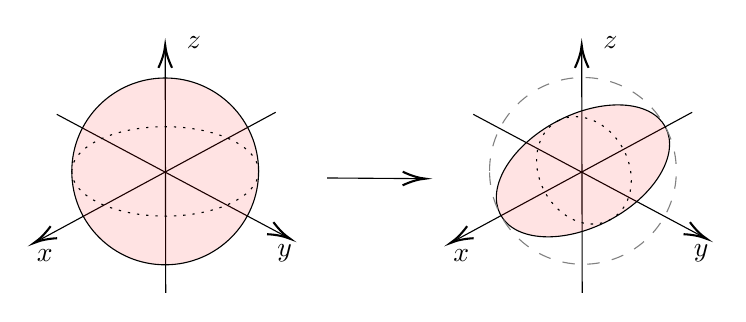
\begin{tikzpicture}[x=0.75pt,y=0.75pt,yscale=-1,xscale=1]
%uncomment if require: \path (0,300); %set diagram left start at 0, and has height of 300

%Straight Lines [id:da6053485398317862] 
\draw    (272,98.67) -- (272.25,216) ;

\draw [shift={(272,96.67)}, rotate = 89.88] [color={rgb, 255:red, 0; green, 0; blue, 0 }  ][line width=0.75]    (10.93,-3.29) .. controls (6.95,-1.4) and (3.31,-0.3) .. (0,0) .. controls (3.31,0.3) and (6.95,1.4) .. (10.93,3.29)   ;
%Straight Lines [id:da5611221177442234] 
\draw    (330.49,189.06) -- (219.75,130) ;

\draw [shift={(332.25,190)}, rotate = 208.07] [color={rgb, 255:red, 0; green, 0; blue, 0 }  ][line width=0.75]    (10.93,-3.29) .. controls (6.95,-1.4) and (3.31,-0.3) .. (0,0) .. controls (3.31,0.3) and (6.95,1.4) .. (10.93,3.29)   ;
%Straight Lines [id:da04556902752065173] 
\draw    (210.51,191.05) -- (325.25,129) ;

\draw [shift={(208.75,192)}, rotate = 331.6] [color={rgb, 255:red, 0; green, 0; blue, 0 }  ][line width=0.75]    (10.93,-3.29) .. controls (6.95,-1.4) and (3.31,-0.3) .. (0,0) .. controls (3.31,0.3) and (6.95,1.4) .. (10.93,3.29)   ;
%Shape: Circle [id:dp37532078739974173] 
\draw  [color={rgb, 255:red, 0; green, 0; blue, 0 }  ,draw opacity=1 ][fill={rgb, 255:red, 255; green, 0; blue, 0 }  ,fill opacity=0.11 ] (227,157.5) .. controls (227,132.65) and (247.15,112.5) .. (272,112.5) .. controls (296.85,112.5) and (317,132.65) .. (317,157.5) .. controls (317,182.35) and (296.85,202.5) .. (272,202.5) .. controls (247.15,202.5) and (227,182.35) .. (227,157.5) -- cycle ;
%Flowchart: Connector [id:dp11532730529723412] 
\draw  [dash pattern={on 0.84pt off 2.51pt}] (227,157.5) .. controls (227,145.6) and (247.15,135.96) .. (272,135.96) .. controls (296.85,135.96) and (317,145.6) .. (317,157.5) .. controls (317,169.4) and (296.85,179.04) .. (272,179.04) .. controls (247.15,179.04) and (227,169.4) .. (227,157.5) -- cycle ;
%Straight Lines [id:da8832418739668391] 
\draw    (472.67,98.67) -- (472.92,216) ;

\draw [shift={(472.67,96.67)}, rotate = 89.88] [color={rgb, 255:red, 0; green, 0; blue, 0 }  ][line width=0.75]    (10.93,-3.29) .. controls (6.95,-1.4) and (3.31,-0.3) .. (0,0) .. controls (3.31,0.3) and (6.95,1.4) .. (10.93,3.29)   ;
%Straight Lines [id:da47617521851544065] 
\draw    (531.15,189.06) -- (420.42,130) ;

\draw [shift={(532.92,190)}, rotate = 208.07] [color={rgb, 255:red, 0; green, 0; blue, 0 }  ][line width=0.75]    (10.93,-3.29) .. controls (6.95,-1.4) and (3.31,-0.3) .. (0,0) .. controls (3.31,0.3) and (6.95,1.4) .. (10.93,3.29)   ;
%Straight Lines [id:da7434156963346557] 
\draw    (411.18,191.05) -- (525.92,129) ;

\draw [shift={(409.42,192)}, rotate = 331.6] [color={rgb, 255:red, 0; green, 0; blue, 0 }  ][line width=0.75]    (10.93,-3.29) .. controls (6.95,-1.4) and (3.31,-0.3) .. (0,0) .. controls (3.31,0.3) and (6.95,1.4) .. (10.93,3.29)   ;
%Shape: Ellipse [id:dp23029244427130813] 
\draw  [fill={rgb, 255:red, 255; green, 0; blue, 0 }  ,fill opacity=0.11 ] (433.5,178.29) .. controls (426.54,165.13) and (438.7,145.05) .. (460.67,133.42) .. controls (482.64,121.8) and (506.09,123.05) .. (513.05,136.2) .. controls (520.01,149.36) and (507.84,169.44) .. (485.88,181.07) .. controls (463.91,192.69) and (440.46,191.44) .. (433.5,178.29) -- cycle ;
%Flowchart: Connector [id:dp6541269736325435] 
\draw  [dash pattern={on 0.84pt off 2.51pt}] (461.22,133.14) .. controls (471.75,127.6) and (485.9,133.8) .. (492.82,146.97) .. controls (499.75,160.14) and (496.82,175.31) .. (486.29,180.85) .. controls (475.76,186.38) and (461.61,180.19) .. (454.69,167.02) .. controls (447.76,153.84) and (450.68,138.68) .. (461.22,133.14) -- cycle ;
%Straight Lines [id:da3885817960263316] 
\draw    (350,160.67) -- (395.33,160.99) ;
\draw [shift={(397.33,161)}, rotate = 180.4] [color={rgb, 255:red, 0; green, 0; blue, 0 }  ][line width=0.75]    (10.93,-3.29) .. controls (6.95,-1.4) and (3.31,-0.3) .. (0,0) .. controls (3.31,0.3) and (6.95,1.4) .. (10.93,3.29)   ;

%Shape: Circle [id:dp7814507360993972] 
\draw  [color={rgb, 255:red, 129; green, 129; blue, 129 }  ,draw opacity=1 ][fill={rgb, 255:red, 255; green, 255; blue, 255 }  ,fill opacity=0 ][dash pattern={on 4.5pt off 4.5pt}] (428.27,157.25) .. controls (428.27,132.39) and (448.42,112.25) .. (473.27,112.25) .. controls (498.13,112.25) and (518.27,132.39) .. (518.27,157.25) .. controls (518.27,182.1) and (498.13,202.25) .. (473.27,202.25) .. controls (448.42,202.25) and (428.27,182.1) .. (428.27,157.25) -- cycle ;

% Text Node
\draw (214,198.17) node   {$x$};
% Text Node
\draw (329.5,197.17) node   {$y$};
% Text Node
\draw (285.9,95.57) node   {$z$};
% Text Node
\draw (414.67,198.17) node   {$x$};
% Text Node
\draw (530.17,197.17) node   {$y$};
% Text Node
\draw (486.57,95.57) node   {$z$};


\end{tikzpicture}
\end{center}

\caption{Rappresentazione geometrica della trasformazione $\rho\mapsto \rho'$ dal punto di vista dei vettori nella sfera di Bloch. Generalmente il processo non è invertibile, e il volume può solo diminuire.\label{fig:affine}}
\end{figure}

\subsection{Canale bit-flip}
Un esempio di canale quantistico è quello che \q{inverte} - tramite l'azione di $\sigma_z$ - un qubit con una certa probabilità $p=|\alpha|^2$, senza fare nulla con probabilità $1-p$:
\begin{align*}
\rho' = S(\rho) = \underbrace{|\alpha|^2}_{p} \sigma_x \rho \sigma_x^\dag + (1-|\alpha|^2) \rho
\end{align*}
Nella rappresentazione di Kraus si trovano:
\begin{align*}
E_0 = \sqrt{1-|\alpha|^2} \bb{I}\qquad E_1 = |\alpha| \sigma_x
\end{align*}

Per esempio, se partiamo da uno stato $\rho = \ket{0}\bra{0}$, otterremo:
\begin{align*}
\rho' = |\alpha|^2 \ket{1}\bra{1} + (1-|\alpha|^2)\ket{0}\bra{0}
\end{align*}

Analogamente:
\begin{align*}
\ket{1}\bra{1} \mapsto \rho0 = |\alpha|^2 \ket{0}\bra{0} + (1-|\alpha|^2)\ket{1}\bra{1}       
\end{align*}

Geometricamente, il bit-flip corrisponde alla trasformazione affine data da:
\begin{align*}
\begin{cases}
x'=x\\
y' = (1-2|\alpha|^2) y\\
z'=(1-2|\alpha|^2)z
\end{cases}
\end{align*}

\begin{figure}[H]
\centering
\begin{center}
\tikzset{every picture/.style={line width=0.75pt}} %set default line width to 0.75pt        

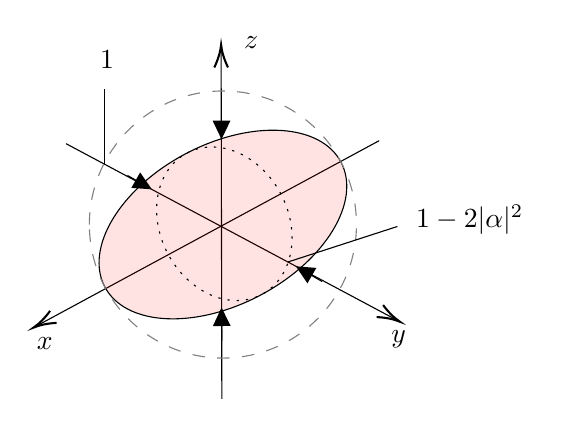
\begin{tikzpicture}[x=0.75pt,y=0.75pt,yscale=-1,xscale=1]
%uncomment if require: \path (0,300); %set diagram left start at 0, and has height of 300

%Straight Lines [id:da4634913670560876] 
\draw    (390.28,89.44) -- (390.63,258.07) ;

\draw [shift={(390.27,87.44)}, rotate = 89.88] [color={rgb, 255:red, 0; green, 0; blue, 0 }  ][line width=0.75]    (10.93,-3.29) .. controls (6.95,-1.4) and (3.31,-0.3) .. (0,0) .. controls (3.31,0.3) and (6.95,1.4) .. (10.93,3.29)   ;
%Straight Lines [id:da7027814771162795] 
\draw    (474.66,219.95) -- (315.56,135.1) ;

\draw [shift={(476.42,220.89)}, rotate = 208.07] [color={rgb, 255:red, 0; green, 0; blue, 0 }  ][line width=0.75]    (10.93,-3.29) .. controls (6.95,-1.4) and (3.31,-0.3) .. (0,0) .. controls (3.31,0.3) and (6.95,1.4) .. (10.93,3.29)   ;
%Straight Lines [id:da054091669678108856] 
\draw    (301.59,222.8) -- (466.41,133.67) ;

\draw [shift={(299.84,223.75)}, rotate = 331.6] [color={rgb, 255:red, 0; green, 0; blue, 0 }  ][line width=0.75]    (10.93,-3.29) .. controls (6.95,-1.4) and (3.31,-0.3) .. (0,0) .. controls (3.31,0.3) and (6.95,1.4) .. (10.93,3.29)   ;
%Shape: Ellipse [id:dp2928278701445042] 
\draw  [fill={rgb, 255:red, 255; green, 0; blue, 0 }  ,fill opacity=0.11 ] (334.27,204.15) .. controls (324.32,185.33) and (341.71,156.61) .. (373.12,140) .. controls (404.54,123.38) and (438.07,125.16) .. (448.02,143.97) .. controls (457.97,162.78) and (440.57,191.5) .. (409.16,208.12) .. controls (377.75,224.73) and (344.22,222.96) .. (334.27,204.15) -- cycle ;
%Flowchart: Connector [id:dp6493116250430526] 
\draw  [dash pattern={on 0.84pt off 2.51pt}] (373.9,139.59) .. controls (388.96,131.67) and (409.19,140.53) .. (419.09,159.36) .. controls (429,178.2) and (424.82,199.89) .. (409.76,207.8) .. controls (394.7,215.72) and (374.47,206.86) .. (364.57,188.03) .. controls (354.66,169.19) and (358.84,147.5) .. (373.9,139.59) -- cycle ;
%Shape: Ellipse [id:dp3865761273050259] 
\draw  [color={rgb, 255:red, 129; green, 129; blue, 129 }  ,draw opacity=1 ][fill={rgb, 255:red, 255; green, 255; blue, 255 }  ,fill opacity=0 ][dash pattern={on 4.5pt off 4.5pt}] (326.8,174.06) .. controls (326.8,138.52) and (355.61,109.71) .. (391.14,109.71) .. controls (426.68,109.71) and (455.49,138.52) .. (455.49,174.06) .. controls (455.49,209.59) and (426.68,238.4) .. (391.14,238.4) .. controls (355.61,238.4) and (326.8,209.59) .. (326.8,174.06) -- cycle ;
%Straight Lines [id:da15573363567805965] 
\draw    (334,109) -- (334,144.67) ;


%Straight Lines [id:da02321959957065589] 
\draw    (390.48,115.96) -- (390.48,130.96) ;
\draw [shift={(390.48,132.96)}, rotate = 270] [fill={rgb, 255:red, 0; green, 0; blue, 0 }  ][line width=0.75]  [draw opacity=0] (8.93,-4.29) -- (0,0) -- (8.93,4.29) -- cycle    ;

%Straight Lines [id:da29250630756305207] 
\draw    (390.67,229.98) -- (390.5,216.03) ;
\draw [shift={(390.48,214.03)}, rotate = 449.32] [fill={rgb, 255:red, 0; green, 0; blue, 0 }  ][line width=0.75]  [draw opacity=0] (8.93,-4.29) -- (0,0) -- (8.93,4.29) -- cycle    ;

%Straight Lines [id:da6013401849188202] 
\draw    (438.95,201.52) -- (428.02,195.19) ;
\draw [shift={(426.29,194.19)}, rotate = 390.07] [fill={rgb, 255:red, 0; green, 0; blue, 0 }  ][line width=0.75]  [draw opacity=0] (8.93,-4.29) -- (0,0) -- (8.93,4.29) -- cycle    ;

%Straight Lines [id:da3830757023018092] 
\draw    (345.18,150.42) -- (355.18,156.1) ;
\draw [shift={(356.91,157.09)}, rotate = 209.6] [fill={rgb, 255:red, 0; green, 0; blue, 0 }  ][line width=0.75]  [draw opacity=0] (8.93,-4.29) -- (0,0) -- (8.93,4.29) -- cycle    ;

%Straight Lines [id:da8885381211089192] 
\draw    (422.46,192.11) -- (475.2,175) ;



% Text Node
\draw (305.34,231.24) node   {$x$};
% Text Node
\draw (475.82,229.14) node   {$y$};
% Text Node
\draw (404.82,86.53) node   {$z$};
% Text Node
\draw (510.04,171.75) node   {$1-2|\alpha |^{2}$};
% Text Node
\draw (335.33,94.67) node   {$1$};


\end{tikzpicture}
\end{center}
\caption{L'operazione di bit-flip deforma la sfera di Bloch contraendola lungo le direzioni $\hat{y}$ e $\hat{z}$ di una quantità $1-2|\alpha|^2$, e lasciandola invariata lungo $\hat{x}$\label{fig:bit-flip-geometrica}}
\end{figure}

\begin{figure}[H]
\centering
\begin{center}
\tikzset{every picture/.style={line width=0.75pt}} %set default line width to 0.75pt        

\begin{tikzpicture}[x=0.75pt,y=0.75pt,yscale=-1,xscale=1]
%uncomment if require: \path (0,300); %set diagram left start at 0, and has height of 300

%Straight Lines [id:da7040370192682079] 
\draw    (250,140) -- (410,140) ;


%Straight Lines [id:da21757855629213352] 
\draw    (250,190) -- (410,190) ;


%Straight Lines [id:da9522157388484667] 
\draw    (330,140) -- (330,190) ;


%Shape: Rectangle [id:dp9105897198770163] 
\draw  [color={rgb, 255:red, 0; green, 0; blue, 0 }  ,draw opacity=1 ][fill={rgb, 255:red, 255; green, 255; blue, 255 }  ,fill opacity=1 ] (313.63,174.5) -- (346.38,174.5) -- (346.38,205.5) -- (313.63,205.5) -- cycle ;

% Text Node
\draw (237,140) node   {$\rho$};
% Text Node
\draw (237,190) node   {$|\psi\rangle_c $};
% Text Node
\draw (330,190) node   {$\sigma _{x}$};


\end{tikzpicture}
\end{center}
\caption{Schema del circuito a gate quantistici equivalente all'operazione di bit-flip\label{fig:bit-flip-gate}}
\end{figure}

\subsection{Canale phase-flip}
Analogamente al bit-flip possiamo considerare l'operazione che inverte la fase relativa di un qubit:
\begin{align*}
\rho' = S(\rho) = |\gamma|^2 \sigma_z \rho \sigma_z^\dag + (1-|\gamma|^2)\rho
\end{align*}

\begin{figure}[H]
\centering
\begin{center}
\tikzset{every picture/.style={line width=0.75pt}} %set default line width to 0.75pt        

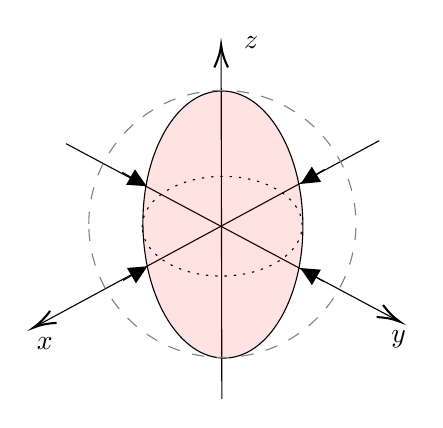
\begin{tikzpicture}[x=0.75pt,y=0.75pt,yscale=-1,xscale=1]
%uncomment if require: \path (0,300); %set diagram left start at 0, and has height of 300

%Straight Lines [id:da4092135086336677] 
\draw    (390.28,89.44) -- (390.63,258.07) ;

\draw [shift={(390.27,87.44)}, rotate = 89.88] [color={rgb, 255:red, 0; green, 0; blue, 0 }  ][line width=0.75]    (10.93,-3.29) .. controls (6.95,-1.4) and (3.31,-0.3) .. (0,0) .. controls (3.31,0.3) and (6.95,1.4) .. (10.93,3.29)   ;
%Straight Lines [id:da913368667683103] 
\draw    (474.66,219.95) -- (315.56,135.1) ;

\draw [shift={(476.42,220.89)}, rotate = 208.07] [color={rgb, 255:red, 0; green, 0; blue, 0 }  ][line width=0.75]    (10.93,-3.29) .. controls (6.95,-1.4) and (3.31,-0.3) .. (0,0) .. controls (3.31,0.3) and (6.95,1.4) .. (10.93,3.29)   ;
%Straight Lines [id:da5556750351058493] 
\draw    (301.59,222.8) -- (466.41,133.67) ;

\draw [shift={(299.84,223.75)}, rotate = 331.6] [color={rgb, 255:red, 0; green, 0; blue, 0 }  ][line width=0.75]    (10.93,-3.29) .. controls (6.95,-1.4) and (3.31,-0.3) .. (0,0) .. controls (3.31,0.3) and (6.95,1.4) .. (10.93,3.29)   ;
%Shape: Ellipse [id:dp2515219920687404] 
\draw  [fill={rgb, 255:red, 255; green, 0; blue, 0 }  ,fill opacity=0.11 ] (392,238.39) .. controls (370.72,238.68) and (353.09,210.1) .. (352.61,174.57) .. controls (352.14,139.04) and (369.01,110) .. (390.29,109.72) .. controls (411.57,109.44) and (429.2,138.01) .. (429.67,173.55) .. controls (430.14,209.08) and (413.28,238.11) .. (392,238.39) -- cycle ;
%Flowchart: Connector [id:dp38456723644805546] 
\draw  [dash pattern={on 0.84pt off 2.51pt}] (352.28,175.27) .. controls (352.14,162.01) and (369.27,151.07) .. (390.55,150.84) .. controls (411.83,150.62) and (429.2,161.19) .. (429.34,174.45) .. controls (429.48,187.72) and (412.34,198.65) .. (391.06,198.88) .. controls (369.78,199.11) and (352.42,188.54) .. (352.28,175.27) -- cycle ;
%Shape: Ellipse [id:dp5510986854592268] 
\draw  [color={rgb, 255:red, 129; green, 129; blue, 129 }  ,draw opacity=1 ][fill={rgb, 255:red, 255; green, 255; blue, 255 }  ,fill opacity=0 ][dash pattern={on 4.5pt off 4.5pt}] (326.53,173.79) .. controls (326.53,138.25) and (355.34,109.45) .. (390.88,109.45) .. controls (426.41,109.45) and (455.22,138.25) .. (455.22,173.79) .. controls (455.22,209.33) and (426.41,238.13) .. (390.88,238.13) .. controls (355.34,238.13) and (326.53,209.33) .. (326.53,173.79) -- cycle ;
%Straight Lines [id:da18253066658130845] 
\draw    (440.1,147.49) -- (430.3,153.45) ;
\draw [shift={(428.6,154.49)}, rotate = 328.66999999999996] [fill={rgb, 255:red, 0; green, 0; blue, 0 }  ][line width=0.75]  [draw opacity=0] (8.93,-4.29) -- (0,0) -- (8.93,4.29) -- cycle    ;

%Straight Lines [id:da11831292961070683] 
\draw    (439.6,201.49) -- (430.21,196.03) ;
\draw [shift={(428.48,195.03)}, rotate = 390.15999999999997] [fill={rgb, 255:red, 0; green, 0; blue, 0 }  ][line width=0.75]  [draw opacity=0] (8.93,-4.29) -- (0,0) -- (8.93,4.29) -- cycle    ;

%Straight Lines [id:da7906756857237944] 
\draw    (343.1,200.99) -- (353.06,195.2) ;
\draw [shift={(354.79,194.19)}, rotate = 509.82] [fill={rgb, 255:red, 0; green, 0; blue, 0 }  ][line width=0.75]  [draw opacity=0] (8.93,-4.29) -- (0,0) -- (8.93,4.29) -- cycle    ;

%Straight Lines [id:da41782602796889634] 
\draw    (342.68,148.92) -- (352.68,154.6) ;
\draw [shift={(354.41,155.59)}, rotate = 209.6] [fill={rgb, 255:red, 0; green, 0; blue, 0 }  ][line width=0.75]  [draw opacity=0] (8.93,-4.29) -- (0,0) -- (8.93,4.29) -- cycle    ;


% Text Node
\draw (305.34,231.24) node   {$x$};
% Text Node
\draw (475.82,229.14) node   {$y$};
% Text Node
\draw (404.82,86.53) node   {$z$};


\end{tikzpicture}

\end{center}
\caption{L'operazione di phase-flip deforma la sfera di Bloch contraendola lungo le direzioni $\hat{x}$ e $\hat{y}$ di una quantità $1-2|\alpha|^2$, e lasciandola invariata lungo $\hat{z}$\label{fig:bit-phaseflip-geometrica}}
\end{figure}


\begin{figure}[H]
\centering
\begin{center}
\tikzset{every picture/.style={line width=0.75pt}} %set default line width to 0.75pt        

\begin{tikzpicture}[x=0.75pt,y=0.75pt,yscale=-1,xscale=1]
%uncomment if require: \path (0,300); %set diagram left start at 0, and has height of 300

%Straight Lines [id:da7040370192682079] 
\draw    (250,140) -- (410,140) ;


%Straight Lines [id:da21757855629213352] 
\draw    (250,190) -- (410,190) ;


%Straight Lines [id:da9522157388484667] 
\draw    (330,140) -- (330,190) ;


%Shape: Rectangle [id:dp9105897198770163] 
\draw  [color={rgb, 255:red, 0; green, 0; blue, 0 }  ,draw opacity=1 ][fill={rgb, 255:red, 255; green, 255; blue, 255 }  ,fill opacity=1 ] (313.63,174.5) -- (346.38,174.5) -- (346.38,205.5) -- (313.63,205.5) -- cycle ;

% Text Node
\draw (237,140) node   {$|\psi \rangle_c $};
% Text Node
\draw (237,190) node   {$\rho$};
% Text Node
\draw (330,190) node   {$\sigma _{z}$};


\end{tikzpicture}
\end{center}
\caption{Schema a gate quantistici dell'operazione di phase-flip (= schema del bit-flip, ma con $\sigma_z$ al posto di $\sigma_x$)\label{fig:phase-flip}}
\end{figure}

\subsection{Canale bit-phase flip}
Mettendo insieme i due canali appena esaminati, consideriamo l'operazione che con una certa probabilità $|\beta|^2 = p$ effettua sia un'inversione del qubit che un'inversione  della sua fase relativa:
 \begin{align*}
\rho'=S(\rho) = |\beta|^2 \sigma_y \rho \sigma_y^\dag + (1-|\beta|^2 )\rho
\end{align*}


\begin{figure}[H]
    \centering
    \begin{center}
\tikzset{every picture/.style={line width=0.75pt}} %set default line width to 0.75pt        

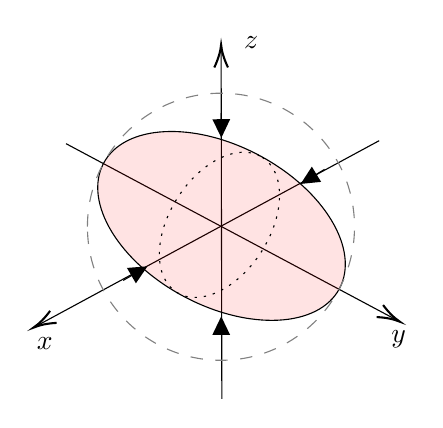
\begin{tikzpicture}[x=0.75pt,y=0.75pt,yscale=-1,xscale=1]
%uncomment if require: \path (0,300); %set diagram left start at 0, and has height of 300

%Straight Lines [id:da04878628540597352] 
\draw    (390.28,89.44) -- (390.63,258.07) ;

\draw [shift={(390.27,87.44)}, rotate = 89.88] [color={rgb, 255:red, 0; green, 0; blue, 0 }  ][line width=0.75]    (10.93,-3.29) .. controls (6.95,-1.4) and (3.31,-0.3) .. (0,0) .. controls (3.31,0.3) and (6.95,1.4) .. (10.93,3.29)   ;
%Straight Lines [id:da7951196053849339] 
\draw    (474.66,219.95) -- (315.56,135.1) ;

\draw [shift={(476.42,220.89)}, rotate = 208.07] [color={rgb, 255:red, 0; green, 0; blue, 0 }  ][line width=0.75]    (10.93,-3.29) .. controls (6.95,-1.4) and (3.31,-0.3) .. (0,0) .. controls (3.31,0.3) and (6.95,1.4) .. (10.93,3.29)   ;
%Straight Lines [id:da3594428403755976] 
\draw    (301.59,222.8) -- (466.41,133.67) ;

\draw [shift={(299.84,223.75)}, rotate = 331.6] [color={rgb, 255:red, 0; green, 0; blue, 0 }  ][line width=0.75]    (10.93,-3.29) .. controls (6.95,-1.4) and (3.31,-0.3) .. (0,0) .. controls (3.31,0.3) and (6.95,1.4) .. (10.93,3.29)   ;
%Shape: Ellipse [id:dp0013257032763898113] 
\draw  [fill={rgb, 255:red, 255; green, 0; blue, 0 }  ,fill opacity=0.11 ] (333.66,144.52) .. controls (343.65,125.73) and (377.19,124.02) .. (408.57,140.7) .. controls (439.94,157.38) and (457.28,186.14) .. (447.29,204.93) .. controls (437.3,223.72) and (403.76,225.43) .. (372.39,208.75) .. controls (341.01,192.06) and (323.67,163.31) .. (333.66,144.52) -- cycle ;
%Flowchart: Connector [id:dp28024248456032863] 
\draw  [dash pattern={on 0.84pt off 2.51pt}] (410.13,141.67) .. controls (421.33,148.78) and (421.16,169.11) .. (409.75,187.07) .. controls (398.34,205.04) and (380.01,213.83) .. (368.82,206.72) .. controls (357.62,199.61) and (357.79,179.28) .. (369.2,161.32) .. controls (380.61,143.35) and (398.93,134.56) .. (410.13,141.67) -- cycle ;
%Shape: Ellipse [id:dp7398465212526404] 
\draw  [color={rgb, 255:red, 129; green, 129; blue, 129 }  ,draw opacity=1 ][fill={rgb, 255:red, 255; green, 255; blue, 255 }  ,fill opacity=0 ][dash pattern={on 4.5pt off 4.5pt}] (325.87,175.12) .. controls (325.87,139.59) and (354.67,110.78) .. (390.21,110.78) .. controls (425.75,110.78) and (454.55,139.59) .. (454.55,175.12) .. controls (454.55,210.66) and (425.75,239.47) .. (390.21,239.47) .. controls (354.67,239.47) and (325.87,210.66) .. (325.87,175.12) -- cycle ;
%Straight Lines [id:da6931867896015693] 
\draw    (440.1,147.49) -- (430.3,153.45) ;
\draw [shift={(428.6,154.49)}, rotate = 328.66999999999996] [fill={rgb, 255:red, 0; green, 0; blue, 0 }  ][line width=0.75]  [draw opacity=0] (8.93,-4.29) -- (0,0) -- (8.93,4.29) -- cycle    ;

%Straight Lines [id:da28818954417416554] 
\draw    (390.33,229.67) -- (390.33,220.33) ;
\draw [shift={(390.33,218.33)}, rotate = 450] [fill={rgb, 255:red, 0; green, 0; blue, 0 }  ][line width=0.75]  [draw opacity=0] (8.93,-4.29) -- (0,0) -- (8.93,4.29) -- cycle    ;

%Straight Lines [id:da21228833563062532] 
\draw    (343.1,200.99) -- (353.06,195.2) ;
\draw [shift={(354.79,194.19)}, rotate = 509.82] [fill={rgb, 255:red, 0; green, 0; blue, 0 }  ][line width=0.75]  [draw opacity=0] (8.93,-4.29) -- (0,0) -- (8.93,4.29) -- cycle    ;

%Straight Lines [id:da5507177558757452] 
\draw    (390.33,120.33) -- (390.4,130.25) ;
\draw [shift={(390.41,132.25)}, rotate = 269.61] [fill={rgb, 255:red, 0; green, 0; blue, 0 }  ][line width=0.75]  [draw opacity=0] (8.93,-4.29) -- (0,0) -- (8.93,4.29) -- cycle    ;


% Text Node
\draw (305.34,231.24) node   {$x$};
% Text Node
\draw (475.82,229.14) node   {$y$};
% Text Node
\draw (404.82,86.53) node   {$z$};


\end{tikzpicture}
\end{center}
    \caption{Canale di Bit-Phase Flip}
    \label{fig:bit-phase-flip}
\end{figure}

\subsection{Depolarizing channel}
Unendo tutte e tre le ultime operazioni (con una certa probabilità $p$) otteniamo il funzionamento del \textbf{depolarizing channel}:
\begin{align*}
\rho' = \frac{1}{3}[\sigma_x \rho \sigma_x^\dag + \sigma_y \rho \sigma_y^\dag + \sigma_z\rho \sigma_z^\dag ] + (1-p)\rho
\end{align*}
dove stiamo usando tutti e $4$ gli operatori di Kraus:
\begin{align*}
E_k = \left\{\sqrt{1-p}\bb{I}, \sqrt{\frac{p}{3}}\sigma_i\right\}
\end{align*}
Geometricamente ciò equivale a una contrazione \textit{lungo tutti gli assi}:
\begin{align*}
\vec{r}' = \left(1-\frac{4}{3}p\right)\vec{r}
\end{align*}
\begin{figure}[H]
\centering
\begin{center}
\tikzset{every picture/.style={line width=0.75pt}} %set default line width to 0.75pt        

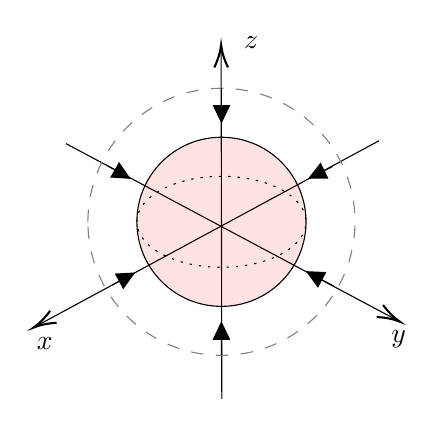
\begin{tikzpicture}[x=0.75pt,y=0.75pt,yscale=-1,xscale=1]
%uncomment if require: \path (0,300); %set diagram left start at 0, and has height of 300

%Straight Lines [id:da6327810677274381] 
\draw    (333.61,60.77) -- (333.96,229.4) ;

\draw [shift={(333.61,58.77)}, rotate = 89.88] [color={rgb, 255:red, 0; green, 0; blue, 0 }  ][line width=0.75]    (10.93,-3.29) .. controls (6.95,-1.4) and (3.31,-0.3) .. (0,0) .. controls (3.31,0.3) and (6.95,1.4) .. (10.93,3.29)   ;
%Straight Lines [id:da43353641222945294] 
\draw    (417.99,191.28) -- (258.9,106.43) ;

\draw [shift={(419.76,192.22)}, rotate = 208.07] [color={rgb, 255:red, 0; green, 0; blue, 0 }  ][line width=0.75]    (10.93,-3.29) .. controls (6.95,-1.4) and (3.31,-0.3) .. (0,0) .. controls (3.31,0.3) and (6.95,1.4) .. (10.93,3.29)   ;
%Straight Lines [id:da29221111629397845] 
\draw    (244.93,194.13) -- (409.75,105) ;

\draw [shift={(243.17,195.08)}, rotate = 331.6] [color={rgb, 255:red, 0; green, 0; blue, 0 }  ][line width=0.75]    (10.93,-3.29) .. controls (6.95,-1.4) and (3.31,-0.3) .. (0,0) .. controls (3.31,0.3) and (6.95,1.4) .. (10.93,3.29)   ;
%Shape: Ellipse [id:dp8570748143920477] 
\draw  [color={rgb, 255:red, 129; green, 129; blue, 129 }  ,draw opacity=1 ][fill={rgb, 255:red, 255; green, 255; blue, 255 }  ,fill opacity=0 ][dash pattern={on 4.5pt off 4.5pt}] (269.44,144.09) .. controls (269.44,108.55) and (298.25,79.74) .. (333.79,79.74) .. controls (369.32,79.74) and (398.13,108.55) .. (398.13,144.09) .. controls (398.13,179.62) and (369.32,208.43) .. (333.79,208.43) .. controls (298.25,208.43) and (269.44,179.62) .. (269.44,144.09) -- cycle ;
%Straight Lines [id:da7627818098470558] 
\draw    (333.79,79.74) -- (333.79,94.74) ;
\draw [shift={(333.79,96.74)}, rotate = 270] [fill={rgb, 255:red, 0; green, 0; blue, 0 }  ][line width=0.75]  [draw opacity=0] (8.93,-4.29) -- (0,0) -- (8.93,4.29) -- cycle    ;

%Straight Lines [id:da26588049811584535] 
\draw    (387.75,175) -- (376.21,168.8) ;
\draw [shift={(374.45,167.86)}, rotate = 388.24] [fill={rgb, 255:red, 0; green, 0; blue, 0 }  ][line width=0.75]  [draw opacity=0] (8.93,-4.29) -- (0,0) -- (8.93,4.29) -- cycle    ;

%Straight Lines [id:da3545162299588869] 
\draw    (278.35,116.75) -- (288.34,122.43) ;
\draw [shift={(290.08,123.42)}, rotate = 209.6] [fill={rgb, 255:red, 0; green, 0; blue, 0 }  ][line width=0.75]  [draw opacity=0] (8.93,-4.29) -- (0,0) -- (8.93,4.29) -- cycle    ;

%Shape: Ellipse [id:dp820204870605332] 
\draw  [color={rgb, 255:red, 0; green, 0; blue, 0 }  ,draw opacity=1 ][fill={rgb, 255:red, 255; green, 0; blue, 0 }  ,fill opacity=0.11 ] (293.04,144.09) .. controls (293.04,121.58) and (311.28,103.34) .. (333.79,103.34) .. controls (356.29,103.34) and (374.53,121.58) .. (374.53,144.09) .. controls (374.53,166.59) and (356.29,184.83) .. (333.79,184.83) .. controls (311.28,184.83) and (293.04,166.59) .. (293.04,144.09) -- cycle ;
%Shape: Ellipse [id:dp7684721210975072] 
\draw  [color={rgb, 255:red, 0; green, 0; blue, 0 }  ,draw opacity=1 ][fill={rgb, 255:red, 255; green, 255; blue, 255 }  ,fill opacity=0 ][dash pattern={on 0.84pt off 2.51pt}] (293.04,144.09) .. controls (293.04,131.98) and (311.28,122.17) .. (333.79,122.17) .. controls (356.29,122.17) and (374.53,131.98) .. (374.53,144.09) .. controls (374.53,156.19) and (356.29,166) .. (333.79,166) .. controls (311.28,166) and (293.04,156.19) .. (293.04,144.09) -- cycle ;
%Straight Lines [id:da42628493241642684] 
\draw    (333.79,208.43) -- (333.75,194) ;
\draw [shift={(333.75,192)}, rotate = 449.87] [fill={rgb, 255:red, 0; green, 0; blue, 0 }  ][line width=0.75]  [draw opacity=0] (8.93,-4.29) -- (0,0) -- (8.93,4.29) -- cycle    ;

%Straight Lines [id:da6914717456344306] 
\draw    (280.85,174.75) -- (290.5,169.46) ;
\draw [shift={(292.25,168.5)}, rotate = 511.26] [fill={rgb, 255:red, 0; green, 0; blue, 0 }  ][line width=0.75]  [draw opacity=0] (8.93,-4.29) -- (0,0) -- (8.93,4.29) -- cycle    ;

%Straight Lines [id:da6813940090017196] 
\draw    (387.25,117.5) -- (377.24,122.47) ;
\draw [shift={(375.45,123.36)}, rotate = 333.6] [fill={rgb, 255:red, 0; green, 0; blue, 0 }  ][line width=0.75]  [draw opacity=0] (8.93,-4.29) -- (0,0) -- (8.93,4.29) -- cycle    ;


% Text Node
\draw (248.68,202.57) node   {$x$};
% Text Node
\draw (419.16,200.47) node   {$y$};
% Text Node
\draw (348.15,57.87) node   {$z$};


\end{tikzpicture}
\end{center}
\caption{Azione del depolarizing channel sulla Sfera di Bloch\label{fig:depolarizing-geom}}
\end{figure}

Applicando diverse volte tale canale è possibile far collassare l'intera sfera di Bloch sull'origine (che è il punto fisso della trasformazione geometrica, e corrisponde a $\vec{r}=\vec{0}\Rightarrow \rho=\bb{I}/2$ - stato massimamente misto).

\subsection{Amplitude damping}
Consideriamo ora l'operazione in rappresentazione di Kraus:
\begin{align*}
\rho'=S(\rho) = E_0 \rho E_0^\dag + E_1 \rho E_1^\dag = \begin{pmatrix}
\rho_{00} + p\rho_{11} & \sqrt{1-p}\rho_{01}\\
\sqrt{1-p}\rho_{10} & (1-p)\rho_{11}\end{pmatrix}
\end{align*}
dove gli operatori di Kraus $\{E_k\}$ sono dati da:
\begin{align*}
E_0 = \begin{pmatrix}1 & 0\\ 0 & \sqrt{1-p}\end{pmatrix} \qquad E_1 = \begin{pmatrix} 0 & \sqrt{p}\\ 0 & 0 \end{pmatrix}
\end{align*}
Tale canale \q{trasferisce} parte della popolazione di $\ket{1}$ a $\ket{0}$. Lo si vede partendo da uno stato eccitato $\ket{1}$:
\begin{align*}
\rho = \ket{1}\bra{1} \mapsto \rho' = p \ket{0}\bra{0} + (1-p) \ket{1}\bra{1}
\end{align*}
Notiamo che tale trasformazione mappa uno stato puro in uno stato misto (dato che è una combinazione lineare di proiettori indipendenti).

\begin{figure}[H]
\centering
\begin{center}
\tikzset{every picture/.style={line width=0.75pt}} %set default line width to 0.75pt        

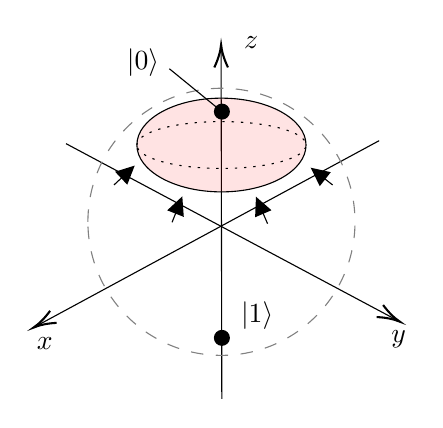
\begin{tikzpicture}[x=0.75pt,y=0.75pt,yscale=-1,xscale=1]
%uncomment if require: \path (0,300); %set diagram left start at 0, and has height of 300

%Straight Lines [id:da46385413602270376] 
\draw    (333.61,60.77) -- (333.96,229.4) ;

\draw [shift={(333.61,58.77)}, rotate = 89.88] [color={rgb, 255:red, 0; green, 0; blue, 0 }  ][line width=0.75]    (10.93,-3.29) .. controls (6.95,-1.4) and (3.31,-0.3) .. (0,0) .. controls (3.31,0.3) and (6.95,1.4) .. (10.93,3.29)   ;
%Straight Lines [id:da07165771898819284] 
\draw    (417.99,191.28) -- (258.9,106.43) ;

\draw [shift={(419.76,192.22)}, rotate = 208.07] [color={rgb, 255:red, 0; green, 0; blue, 0 }  ][line width=0.75]    (10.93,-3.29) .. controls (6.95,-1.4) and (3.31,-0.3) .. (0,0) .. controls (3.31,0.3) and (6.95,1.4) .. (10.93,3.29)   ;
%Straight Lines [id:da788321011372886] 
\draw    (244.93,194.13) -- (409.75,105) ;

\draw [shift={(243.17,195.08)}, rotate = 331.6] [color={rgb, 255:red, 0; green, 0; blue, 0 }  ][line width=0.75]    (10.93,-3.29) .. controls (6.95,-1.4) and (3.31,-0.3) .. (0,0) .. controls (3.31,0.3) and (6.95,1.4) .. (10.93,3.29)   ;
%Shape: Ellipse [id:dp20286413736066145] 
\draw  [color={rgb, 255:red, 129; green, 129; blue, 129 }  ,draw opacity=1 ][fill={rgb, 255:red, 255; green, 255; blue, 255 }  ,fill opacity=0 ][dash pattern={on 4.5pt off 4.5pt}] (269.44,144.09) .. controls (269.44,108.55) and (298.25,79.74) .. (333.79,79.74) .. controls (369.32,79.74) and (398.13,108.55) .. (398.13,144.09) .. controls (398.13,179.62) and (369.32,208.43) .. (333.79,208.43) .. controls (298.25,208.43) and (269.44,179.62) .. (269.44,144.09) -- cycle ;
%Straight Lines [id:da9846078434540908] 
\draw    (282,126.33) -- (290.54,118.36) ;
\draw [shift={(292,117)}, rotate = 496.97] [fill={rgb, 255:red, 0; green, 0; blue, 0 }  ][line width=0.75]  [draw opacity=0] (8.93,-4.29) -- (0,0) -- (8.93,4.29) -- cycle    ;

%Shape: Ellipse [id:dp1318399329259652] 
\draw  [color={rgb, 255:red, 0; green, 0; blue, 0 }  ,draw opacity=1 ][fill={rgb, 255:red, 255; green, 0; blue, 0 }  ,fill opacity=0.11 ] (293.04,107.09) .. controls (293.04,94.62) and (311.28,84.51) .. (333.79,84.51) .. controls (356.29,84.51) and (374.53,94.62) .. (374.53,107.09) .. controls (374.53,119.56) and (356.29,129.67) .. (333.79,129.67) .. controls (311.28,129.67) and (293.04,119.56) .. (293.04,107.09) -- cycle ;
%Shape: Ellipse [id:dp5367854055187202] 
\draw  [color={rgb, 255:red, 0; green, 0; blue, 0 }  ,draw opacity=1 ][fill={rgb, 255:red, 255; green, 255; blue, 255 }  ,fill opacity=0 ][dash pattern={on 0.84pt off 2.51pt}] (293.04,107.09) .. controls (293.04,100.85) and (311.28,95.8) .. (333.79,95.8) .. controls (356.29,95.8) and (374.53,100.85) .. (374.53,107.09) .. controls (374.53,113.32) and (356.29,118.38) .. (333.79,118.38) .. controls (311.28,118.38) and (293.04,113.32) .. (293.04,107.09) -- cycle ;
%Straight Lines [id:da6133901751266062] 
\draw    (356,145) -- (351.21,133.84) ;
\draw [shift={(350.42,132)}, rotate = 426.76] [fill={rgb, 255:red, 0; green, 0; blue, 0 }  ][line width=0.75]  [draw opacity=0] (8.93,-4.29) -- (0,0) -- (8.93,4.29) -- cycle    ;

%Straight Lines [id:da5433580038865533] 
\draw    (310,144.33) -- (314.18,133.69) ;
\draw [shift={(314.92,131.83)}, rotate = 471.47] [fill={rgb, 255:red, 0; green, 0; blue, 0 }  ][line width=0.75]  [draw opacity=0] (8.93,-4.29) -- (0,0) -- (8.93,4.29) -- cycle    ;

%Straight Lines [id:da29998739050710443] 
\draw    (387.33,126.33) -- (378.36,119.26) ;
\draw [shift={(376.79,118.02)}, rotate = 398.23] [fill={rgb, 255:red, 0; green, 0; blue, 0 }  ][line width=0.75]  [draw opacity=0] (8.93,-4.29) -- (0,0) -- (8.93,4.29) -- cycle    ;

%Straight Lines [id:da5972570395205128] 
\draw    (334,91) ;

\draw [shift={(334,91)}, rotate = 0] [color={rgb, 255:red, 0; green, 0; blue, 0 }  ][fill={rgb, 255:red, 0; green, 0; blue, 0 }  ][line width=0.75]      (0, 0) circle [x radius= 3.35, y radius= 3.35]   ;
%Straight Lines [id:da8015106471658033] 
\draw    (308.67,70.33) -- (334,91) ;


%Straight Lines [id:da31223773331739313] 
\draw    (334,200) ;

\draw [shift={(334,200)}, rotate = 0] [color={rgb, 255:red, 0; green, 0; blue, 0 }  ][fill={rgb, 255:red, 0; green, 0; blue, 0 }  ][line width=0.75]      (0, 0) circle [x radius= 3.35, y radius= 3.35]   ;

% Text Node
\draw (248.68,202.57) node   {$x$};
% Text Node
\draw (419.16,200.47) node   {$y$};
% Text Node
\draw (348.15,57.87) node   {$z$};
% Text Node
\draw (296,67.33) node   {$|0\rangle $};
% Text Node
\draw (351,189.33) node   {$|1\rangle $};


\end{tikzpicture}
\end{center}
\caption{Schema grafico del canale di amplitude damping: la sfera di Bloch viene contratta verso il punto corrispondente allo stato $\ket{0}\bra{0}$ \label{fig:damping-schema}}
\end{figure}

Applicando $n$ volte di seguito l'azione del canale si trova:
\begin{align*}
\rho_{11}^{(n)} = (1-p)^n \rho_{11}^(0) = e^{n\ln(1-p)}\rho_{11} \xrightarrow[n\to\infty]{} \ket{0}\bra0
\end{align*}

\textbf{Nota}: tutto ciò è molto diverso dall'azione di un gate NOT, che è un processo coerente (trasforma stati puri in stati puri mediante l'evoluzione unitaria). D'altro canto l'amplitude damping è intrinsecamente incoerente: nel corso del \textit{flip} vengono attraversati infiniti stati misti (rappresentati da punti interni alla sfera di Bloch).


\begin{figure}
    \centering
    \begin{center}
\tikzset{every picture/.style={line width=0.75pt}} %set default line width to 0.75pt        

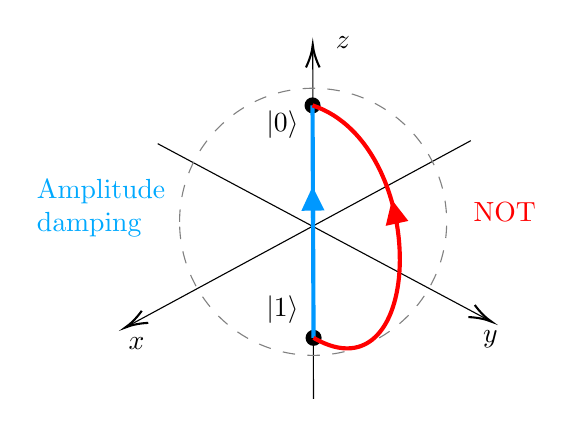
\begin{tikzpicture}[x=0.75pt,y=0.75pt,yscale=-1,xscale=1]
%uncomment if require: \path (0,300); %set diagram left start at 0, and has height of 300

%Straight Lines [id:da7737503638770256] 
\draw    (333.61,60.77) -- (333.96,229.4) ;

\draw [shift={(333.61,58.77)}, rotate = 89.88] [color={rgb, 255:red, 0; green, 0; blue, 0 }  ][line width=0.75]    (10.93,-3.29) .. controls (6.95,-1.4) and (3.31,-0.3) .. (0,0) .. controls (3.31,0.3) and (6.95,1.4) .. (10.93,3.29)   ;
%Straight Lines [id:da036399788845072445] 
\draw    (417.99,191.28) -- (258.9,106.43) ;

\draw [shift={(419.76,192.22)}, rotate = 208.07] [color={rgb, 255:red, 0; green, 0; blue, 0 }  ][line width=0.75]    (10.93,-3.29) .. controls (6.95,-1.4) and (3.31,-0.3) .. (0,0) .. controls (3.31,0.3) and (6.95,1.4) .. (10.93,3.29)   ;
%Straight Lines [id:da43723008785600936] 
\draw    (244.93,194.13) -- (409.75,105) ;

\draw [shift={(243.17,195.08)}, rotate = 331.6] [color={rgb, 255:red, 0; green, 0; blue, 0 }  ][line width=0.75]    (10.93,-3.29) .. controls (6.95,-1.4) and (3.31,-0.3) .. (0,0) .. controls (3.31,0.3) and (6.95,1.4) .. (10.93,3.29)   ;
%Shape: Ellipse [id:dp040611550098602844] 
\draw  [color={rgb, 255:red, 129; green, 129; blue, 129 }  ,draw opacity=1 ][fill={rgb, 255:red, 255; green, 255; blue, 255 }  ,fill opacity=0 ][dash pattern={on 4.5pt off 4.5pt}] (269.44,144.09) .. controls (269.44,108.55) and (298.25,79.74) .. (333.79,79.74) .. controls (369.32,79.74) and (398.13,108.55) .. (398.13,144.09) .. controls (398.13,179.62) and (369.32,208.43) .. (333.79,208.43) .. controls (298.25,208.43) and (269.44,179.62) .. (269.44,144.09) -- cycle ;
%Straight Lines [id:da9111458785738127] 
\draw    (333.5,88) ;

\draw [shift={(333.5,88)}, rotate = 0] [color={rgb, 255:red, 0; green, 0; blue, 0 }  ][fill={rgb, 255:red, 0; green, 0; blue, 0 }  ][line width=0.75]      (0, 0) circle [x radius= 3.35, y radius= 3.35]   ;
%Straight Lines [id:da49656140173216756] 
\draw    (334,200) ;

\draw [shift={(334,200)}, rotate = 0] [color={rgb, 255:red, 0; green, 0; blue, 0 }  ][fill={rgb, 255:red, 0; green, 0; blue, 0 }  ][line width=0.75]      (0, 0) circle [x radius= 3.35, y radius= 3.35]   ;
%Straight Lines [id:da07421071884762709] 
\draw [color={rgb, 255:red, 0; green, 152; blue, 255 }  ,draw opacity=1 ][line width=1.5]    (334,200) -- (333.5,88) ;


%Curve Lines [id:da3620807859739079] 
\draw [color={rgb, 255:red, 255; green, 0; blue, 0 }  ,draw opacity=1 ][line width=1.5]    (334,200) .. controls (388.25,231.5) and (390.75,107) .. (333.5,88) ;


%Straight Lines [id:da015392849030563927] 
\draw [color={rgb, 255:red, 0; green, 152; blue, 255 }  ,draw opacity=1 ][line width=1.5]    (333.79,144.09) -- (333.58,130.09) ;
\draw [shift={(333.54,127.09)}, rotate = 449.16] [fill={rgb, 255:red, 0; green, 152; blue, 255 }  ,fill opacity=1 ][line width=1.5]  [draw opacity=0] (11.61,-5.58) -- (0,0) -- (11.61,5.58) -- cycle    ;

%Straight Lines [id:da08770681582068884] 
\draw [color={rgb, 255:red, 255; green, 0; blue, 0 }  ,draw opacity=1 ][line width=1.5]    (374.25,145) -- (372.39,136.43) ;
\draw [shift={(371.75,133.5)}, rotate = 437.74] [fill={rgb, 255:red, 255; green, 0; blue, 0 }  ,fill opacity=1 ][line width=1.5]  [draw opacity=0] (11.61,-5.58) -- (0,0) -- (11.61,5.58) -- cycle    ;


% Text Node
\draw (248.68,202.57) node   {$x$};
% Text Node
\draw (419.16,200.47) node   {$y$};
% Text Node
\draw (348.15,57.87) node   {$z$};
% Text Node
\draw (319,186.33) node   {$|1\rangle $};
% Text Node
\draw (319,97.33) node   {$|0\rangle $};
% Text Node
\draw (426.13,139.59) node [color={rgb, 255:red, 255; green, 0; blue, 0 }  ,opacity=1 ] [align=left] {NOT};
% Text Node
\draw (231.63,137.59) node [color={rgb, 255:red, 0; green, 169; blue, 255 }  ,opacity=1 ] [align=left] {Amplitude\\damping};


\end{tikzpicture}
\end{center}
    \caption{Azione asintotica del canale di Amplitude Damping}
    \label{fig:amplitude-damp-asintoto}
\end{figure}

\subsection{Phase Damping}
L'analogo per le fasi dell'amplitude damping è detto \textbf{phase-damping}.\\
\begin{comment}
\begin{figure}[H]
\centering
[Missing]
\caption{Rappresentazione geometrica dell'azione del canale phase damping\label{fig:phase-damping-geom}}
\end{figure}
\end{comment}
L'idea è di effettuare una successione di phase-shift, i cui angoli $\theta$ sono selezionati con una certa probabilità. Fisicamente ciò corrisponde al caso di una particella in un campo magnetico oscillante.

\begin{align*}
R_z(\theta) = \begin{pmatrix}e^{-i\theta/2} & 0\\ 0 & e^{i\theta/2}\end{pmatrix} \qquad p(\theta) = \frac{1}{\pi\lambda} \exp\left(-\frac{\theta^2}{4\lambda}\right)
\end{align*}

La trasformazione di $\rho'$ è quindi data da una \textit{media} sui vari angoli:
\begin{align*}
\rho' = \int_{-\infty}^{+\infty} d\theta \, \rho(\theta) R_z(\theta) \rho R_z^\dag(\theta) \qquad \rho=\begin{pmatrix}
p & \alpha\\
\alpha^* & 1-p
\end{pmatrix}
\end{align*}

(Nota: gli estremi dell'integrale sono scelti in modo da rendere l'integrazione della gaussiana fattibile analiticamente)\\

Integrando elemento per elemento si giunge a:
\begin{align*}
\rho'= \begin{pmatrix} p & \alpha e^{-\lambda}\\
\alpha^*e^{-\lambda} & 1-p \end{pmatrix}
\end{align*}
che corrisponde al phase-shift channel ponendo $1-2|\gamma|^2 = e^{-\lambda}$. Analogamente a quanto accade con l'amplitude damping, perciò, il phase damping esegue, su tempi lunghi, l'inversione della fase relativa del qubit in esame (tramite un processo non unitario che passa attraverso infiniti stati misti.


\subsection{Canali a 2 qubit}
Un esempio di canali a 2 qubit è dato dall'operazione che \textit{distrugge} l'entanglement. Partiamo per esempio da uno stato di Bell:
\begin{align*}
\ket{\psi^+} = \frac{1}{\sqrt{2}}(\ket{01}+\ket{10}) \Rightarrow \rho=\frac{1}{2}\left(
\begin{array}{cc|cc}
0 & 0 & 0 & 0\\
0 & 1 & \hlc{Yellow}{1} & 0\\ \hline
0 & \hlc{Yellow}{1} & 1 & 0\\
0 & 0 & 0 & 0
\end{array}
\right)
\end{align*}
dove la matrice $\rho$ è espressa nella base computazionale $\{\ket{00}, \ket{01}, \ket{10}, \ket{11}\}$.\\
L'idea di \textit{distruggere l'entanglement} sta nell'annullare i termini fuori dalla diagonale (evidenziati).\\
Notiamo che $\ket{\psi^+}$ è uno stato puro: lo si vede dalla costruzione, oppure dal fatto che la matrice $\op{ker}(\rho-\lambda \bb{I})$ è costituito da un solo vettore (cosa che equivale a dire che $\rho$ ha un solo autovettore).\\

Consideriamo allora un canale in rappresentazione di Kraus:
\begin{align*}
\rho' = \sum F_i \rho F_i^\dag = \frac{1}{2}\left(
\begin{array}{cc|cc}
0 & 0 & 0 & 0\\ 
0 & 1 & \cos\theta & 0\\ \hline
0 & \cos\theta & 1 & 0\\
0 & 0 & 0 & 0
\end{array}
\right)
\end{align*}
con gli operatori di Kraus:
\begin{align*}
F_0 &= \bb{I} \otimes \tilde{F}_0 = \bb{I}\otimes \begin{pmatrix} 1 & 0\\ 0 & \cos\theta\end{pmatrix}\\
F_1 &= \bb{I}\otimes \tilde{F}_1 = \bb{I}\otimes \begin{pmatrix}1 & 0\\ 0 & \sin\theta\end{pmatrix}
\end{align*}
Ponendo $\cos\theta = 0$ si trova:
\begin{align*}
\rho' = \frac{1}{2}\left(
\begin{array}{cc|cc}
0 & 0 & 0 & 0\\ 
0 & 1 & 0 & 0\\ \hline
0 & 0 & 1 & 0\\
0 & 0 & 0 & 0
\end{array}
\right) = \frac{1}{2}\ket{01}\bra{01} + \frac{1}{2}\ket{10}\bra{10}
\end{align*}
che è uno \textbf{stato misto} (somma di proiettori indipendenti).\\

Se osserviamo l'evoluzione dal punto di vista delle matrici ridotte, troviamo:
\begin{align*}
\rho_2 = \underset{1}{\op{Tr}}\rho = \frac{1}{2}\bb{I}\Rightarrow \rho_2' = \underset{1}{\op{Tr}}\rho = \frac{1}{2}\bb{I}
\end{align*}
In altre parole, osservando i singoli qubit non si vede nessun cambiamento. Sono infatti le \textit{correlazioni} tra i due qubit che vengono distrutte: se $\rho$ può essere utilizzata per un trasporto quantistico, $\rho'$ non può esserlo - i due qubit nello stato finale sono completamente indipendenti uno dall'altro.

\section{Master equation}
\marginpar{\danger Parte non ancora ricontrollata}
Consideriamo un'evoluzione temporale infinitesimale:
\begin{align*}
\rho(t+dt) = S(t,t+dt) \rho(t) = \sum_{k=0}^{M-1} E_k \rho(t) E_k^\dag
\end{align*}
con $M \leq N^2$, $N=\op{dim}(\hs)$. Richiediamo le seguenti condizioni:
\begin{enumerate}
\item L'evoluzione per tempi nulli non cambi niente: $S(t;t) = \bb{I}$
\item $S(t,t+dt)$ riproduca i risultati standard dell'equazione di Schr\"odinger dipendente dal tempo nel caso di un'evoluzione unitaria
\item Valga la condizione per la rappresentazione di Kraus:
\begin{align*}
\sum_k E_k^\dag E_k = \bb{I}
\end{align*}
\end{enumerate}

Imponendo tali condizioni si possono determinare le $\{E_k\}$:
\begin{align*}
E_0 &= \bb{I} + \frac{1}{\hbar}(-i\hat{H}+K)dt\\
E_k &= \sqrt{dt} L_k
\end{align*}
Dalla condizione $3$ deve valere:
\begin{align*}
&\left[\bb{I}+\frac{1}{\hbar}(iH+K)dt \right]\left[\bb{I}+\frac{1}{\hbar}(-iH+K)dt\right]+\sum L_k^\dag L_k = \bb{I}\\
\underset{(a)}{\approx} & \frac{2}{\hbar}K\,dt + \sum L_k^\dag L_k\,dt + O([dt]^2) = 0 \Rightarrow K = -\frac{\hbar}{2} \sum_{k=1}^{M-1}L_k^\dag L_k 
\end{align*}
dove in (a) espandiamo al primo ordine.\\

Sostituendo nell'espressione iniziale:
\begin{align*}
\rho(t+dt)=\rho(t) - \frac{i}{\hbar}[H,\rho(t)]dt + \sum \left( L_k \rho L_k^\dag - \frac{1}{2}L_k^\dag L_k\rho(t) - \frac{1}{2}\rho(t) L_k^\dag L_k \right)dt + O([dt]^2)
\end{align*}
dove la prima parte è data dall'equazione di Heisenberg per l'evoluzione temporale, a cui aggiungiamo un termine che la generalizza.\\

Da:
\begin{align*}
\rho(t+dt) = \rho(t) + \rho(t)dt + O([dt]^2)
\end{align*}
Uguagliando le due espressioni troviamo la forma principale della master equation, detta anche equazione di \textit{Gorini-Kossakawski-Sudarshan-Lindblad}:
\begin{align*}
\dot{\rho} = -\frac{i}{\hbar}[H,\rho] + \sum \left(L_k \rho L_k^\dag - \frac{1}{2}L_k^\dag L_k\rho - \frac{1}{2}\rho L_k^\dag K_k\right)
\end{align*}
dove stiamo assumendo che l'ambiente rimanga in un certo stato stazionario, che non può essere modificato dal comportamento del sistema (che è estramemente piccolo rispetto all'ambiente). (Ipotesi di ambiente senza memoria)\\

Un'altra forma per la stessa equazione è data da:
\begin{align*}
\rho = +\frac{i}{\hbar}[H,\rho] + \frac{1}{2}\sum_{i,j=1}^{N^2-1} A_{ij}\left\{[\sigma_i, \rho\sigma_j^\dag] + [\sigma_i\rho, \sigma_j^\dag]\right\}
\end{align*}
dove $A$ è una matrice positiva, $\{\sigma_i\}$ è la base dele matrici Hermitiane, con:
\begin{align*}
\sigma_0 = \frac{\bb{I}}{\sqrt{N}} \qquad \op{Tr}(\sigma_i)=0 \quad i > 0 \qquad \op{Tr}(\sigma_i^\dag \sigma_j) = \delta_{ij}
\end{align*}
(Non dimostreremo l'equivalenza delle due forme)\\


\end{document}


